\chapter{Introduction}


\begin{wrapfigure}{r}{0.4\textwidth}
	\centering
	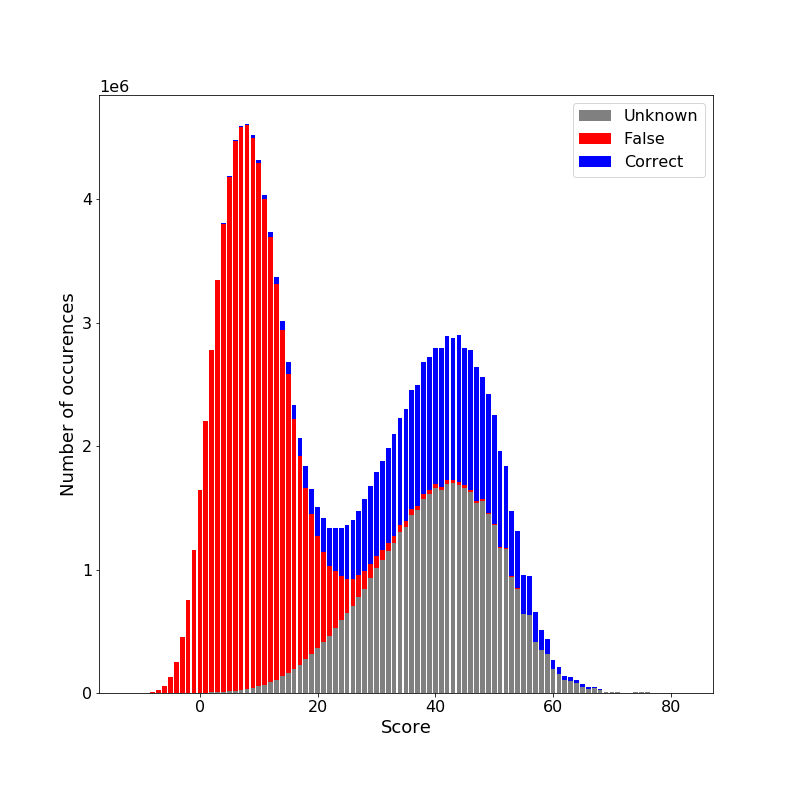
\includegraphics[width=0.5\textwidth]{images/w_3-d_7-hist.png}
	\caption{Spaced word match histogram for pattern set with weight three and seven \textit{Don't Care} positions on \bb data. Source: \cite{hundt2020praktkium}}
	\label{fig:spamogram}
\end{wrapfigure}

Newer, more cost effective and efficient, sequencing methods lead to an ever increasing amount of sequence data being generated \cite{muir2016real}. Due to the problem of aligning $N$ sequences optimally being NP-complete \cite{Russell2016}, there is a strong need for algorithms and heuristics which are able to process large amounts of data faster than current methods. In the space of phylogeny reconstruction this resulted in a new class of methods referred to as "alignment-free" \cite{leimeister2014fast, leimeister2017fast, leimeister2018accurate}. Among them is the \textit{FSWM}, \textbf{F}iltered \textbf{S}paced \textbf{W}ord \textbf{M}atches, approach by Leimeister et al. \cite{leimeister2014fast}. It is based on the idea to define a pattern of \textit{Match} and \textit{Don't Care} positions which is slid over the input sequences, resulting in spaced words comprised of the residues at the \textit{Match} positions and a wildcard character "*" at the \textit{Don't Care} positions. Two equal spaced words constitute a spaced word match. It is these matches, which can also be viewed as a micro alignment of segments in the input sequences, that are the basis for the alignment algorithm proposed in the preliminary work to this thesis \cite{hundt2020praktkium}. The hypothesis being: a complete sequence alignment could be established by finding these micro alignments, assigning a score to each of them and then greedily adding them to a growing alignment. Additionally to proposing an algorithm based on spaced word matches, the preliminary work also evaluated the feasibility of it by examining the distribution of matches on the \bb dataset with respect to their score. As can be seen in figure \ref{fig:spamogram}, a high scoring spaced word match is likely to be correct while those with a low score are most often incorrect. The "correctness" of these matches representing micro alignments was defined in terms of known \textit{core blocks}, necessitating the third option "Unknown" for an alignment of sites of which neither one is part of a core block.



%Multiple sequence alignments are of fundamental importance for a myriad of tasks in the area
%of bioinformatics and biology. They are used for problems such as genomic annotation, protein
%structure annotation or in fields like functional genomics [1]. An exponential increase in sequencing
%data [2] necessitates ever faster alignment methods.
%This report proposes a multiple sequence alignment algorithm which builds upon the DIALIGN [3],
%GABIOS-LIB [4, 5] and FSWM [6] algorithms. In order to examine the feasibility of the approach,
%spaced word matches are systematically evaluated on the BAliBASE version 3 dataset. In particular,
%precision, recall and F 1 values are computed to estimate how "good" spaced word matches are.
%Whereas DIALIGN and GABIOS-LIB are methods for aligning multiple sequences or maintaining
%consistency bounds, FSWM is normally used for phylogenetic distance estimation.